\documentclass{article}

\usepackage[T1]{fontenc}
\usepackage[utf8]{inputenc}
\usepackage[french,english]{babel}

%% This package is necessary to use \includegraphics.
\usepackage{graphicx}

%% This package is necessary to define hyperlinks.
\usepackage{hyperref}

%% These packages are necessary to include code.
\usepackage{listings}
\usepackage{minted} % colored

%% This package is needed to enchance mathematical formulas.
\usepackage{amsmath}



% This is a comment line in latex

% Latex allows you to define your own "commands",
% better known as "macros" in the Latex world.
% The following line is an example of such definition.
\newcommand{\latex}{\LaTeX}


% The next lines contain some meta informations about this document.

\title{Rapport Projet Long\\ Pour le 15 mars 2023}
%\subtitle{A minimal demonstration of \latex}

\author{Ange Herman KOUE-HEMAZRO, Eric Nzaba}


%% Here we begin giving the actual content o the document.
\begin{document}
\maketitle

\selectlanguage{french}

\section{Introduction}
\paragraph{But du projet.} Implémenter une IA pour le jeu d'echecs basée sur la Recherche 
arborescente Monte-Carlo.

\paragraph{Métrique.} On utilise l'api de lichess.org pour la partie graphique de notre projet et
l'api donne aussi la possibilité de jouer contre une IA (niveaux entre 1 et 8) basée sur l'alogythme de stockfish qui est
un des plus puissant qui n'utilise pas les réseaux de neuronnes. Notre projet sera un succès si notre
IA arrive à battre au moins les 3 premiers niveaux de stockfish. Vu que l'algorythme de Monte Carlo
se base sur une simulation de coup pris au hasard, ce sera dur de battre les niveaux supérieur
de stockfish. Du coup le but sera de faire plusieurs simulations de parties contre stockfish et on sortir
les resultats sous forme de pourcentage.

\section{Implementation}
\paragraph{Comment on réalise notre projet.} Nous codons en python et comme dis plus haut, on utilise
l'api de lichess.org pour ne pas avoir à coder la partie graphique du jeu. 

\paragraph{Logiciel déjà codé} . Nous avons déja codé la representation du jeu d'échec ainsi
que les mouvements des pièces mais nous avons encore quelques bugs à régler du coté du roi.
.Nous avons déja fait la connexion avec l'api et codé la partie de l'api qui va nous permettre de jouer
des coups. L'algorythme de monte carlo a déjà été implémenté aussi.

\paragraph{Structure en modules/packages.} Nous avons 3 packages sans compter le package des tests. Le
package {\tt ai} est celui qui contient les fichiers en rapport avec notre IA basé sur Monte Carlo. Le package
{\tt api} quand à lui contiens tout ce qui est en rapport avec l'api de lichess.org, les fonctions de connexions,
de récupération er d'envoie de données etc. Enfin le package {\tt chess} contient tout ce qui est en rapport avec
notre representaion du jeu d'echecs, les fonctions pour avoir tous les coups possibles etc ...

\paragraph{Représentation des données.} Nous avons representé le plateau de jeu comme un tableau d'entier
pour que ca prenne le moins de place que possible dans la mémoire vu que notre algorythme de recherche
passera par des milliers de plateau de jeu. Nous comptons aussi introduire plus tard fichier pour
stocker les mouvements de debut de game comme celui qui permet de liberer le fou ou la reine.

\paragraph{Technologies sur lesquelles notre code s'appuie.} Notre IA se base sur l'algorythme de recherche
arborescente Monte Carlo et nous utilisons aussi l'api de lichess.org pour la partie graphique.

\section{Jalons}
\paragraph{Tâches à realiser pour conclure le projet.} 
\begin{enumerate}
  \item Regler les bugs dans les mouvements des pièces
  \item Permettre à un utilisateur lambda de jouer contre notre IA
\end{enumerate}

\paragraph{Organisation temporelle des tâches.}
\begin{figure}[h]
  \label{fig:geant}
  \hrulefill
  \begin{center}
  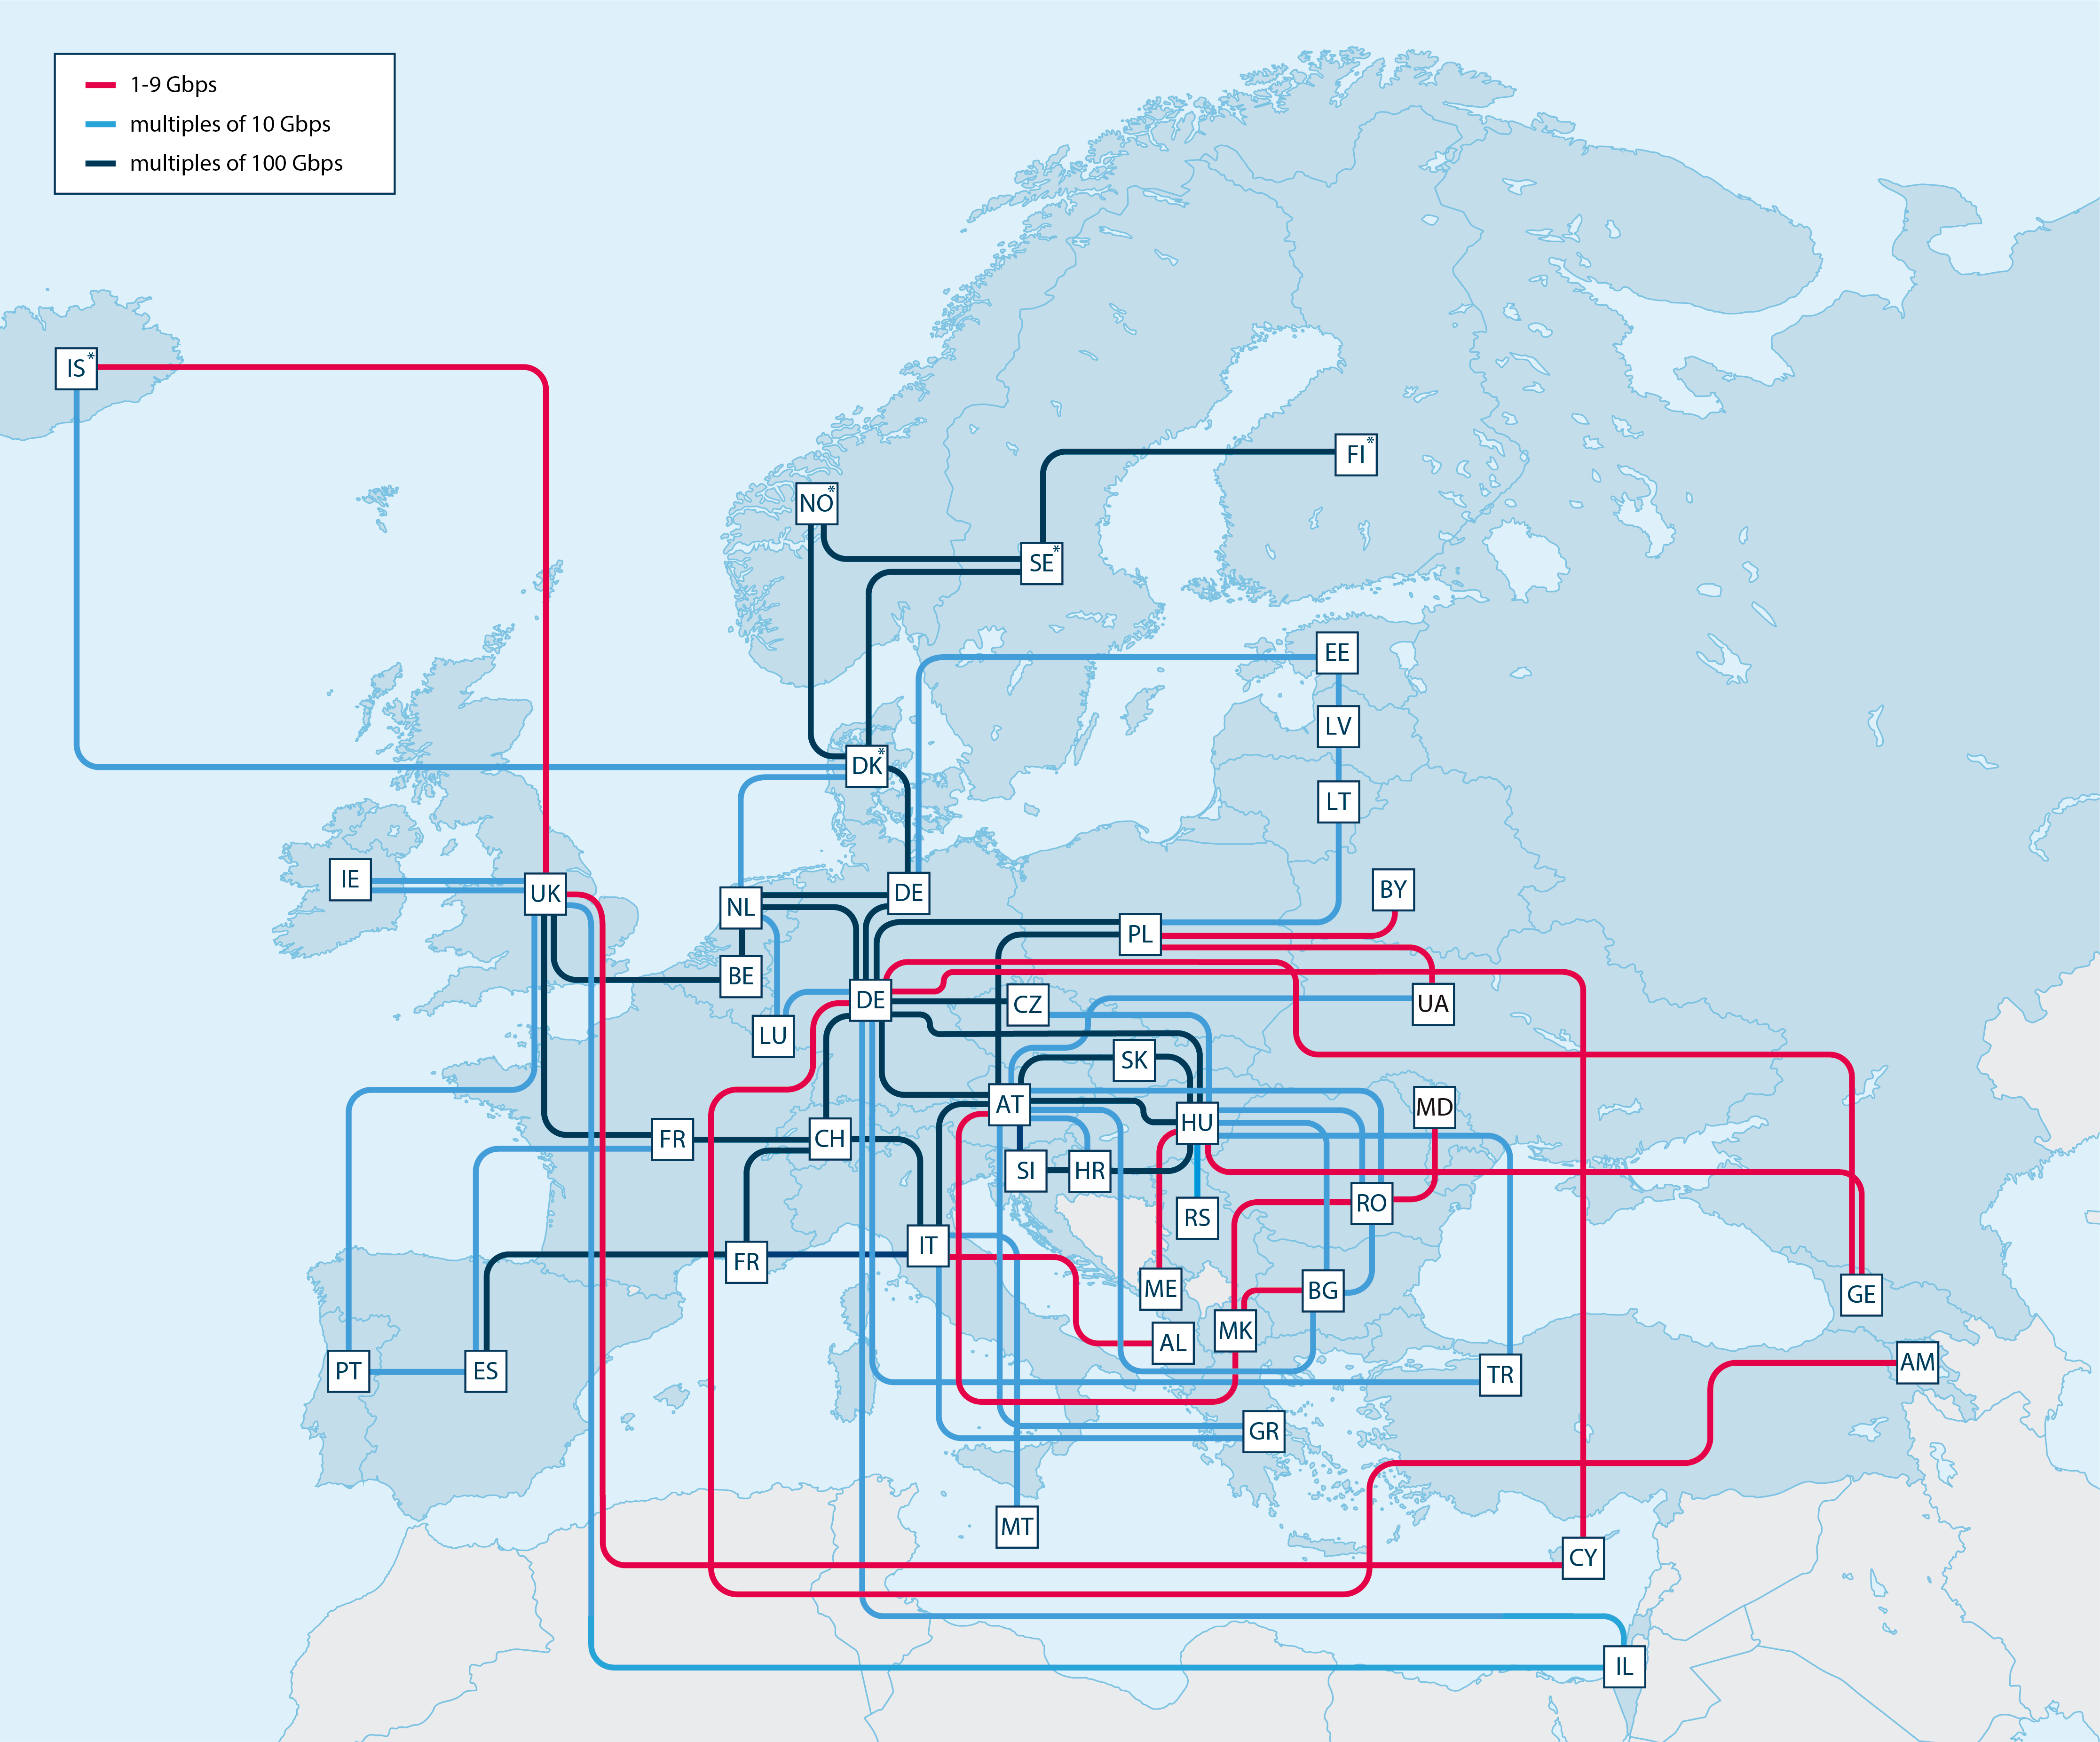
\includegraphics[height=123px,width=180px]{geant}
  \end{center}
  \caption{A picture of the GEANT network.}
  \hrulefill
\end{figure}



\paragraph{Tâches déja terminées.}
\begin{enumerate}
  \item Partie de l'api qui permet à notre IA de jouer contre celles de lichess
  \item Implémentation de l'algorythme de recherche arborescente Monte Carlo
  \item Implémentaion des mouvements d'échecs sauf celui du roi ( Encore quelques bugs)
\end{enumerate}

\end{document}
